% Figure 10: editable LaTeX layout matching Figure 9.
% \figtenpanelwidth is the final size; no outer scaling is applied.
\begin{figure}[!ht]
    \centering
    \begingroup
    \newlength{\figtenpanelwidth}
    \newlength{\figtenlegendunit}
    \setlength{\figtenpanelwidth}{1.55in}
    \setlength{\figtenlegendunit}{\dimexpr\figtenpanelwidth*10/52\relax}

    % Exact RGB values sampled from the updated CFD-Post legend.
    \definecolor{figtenTemp0}{RGB}{70,94,207}
    \definecolor{figtenTemp1}{RGB}{103,136,238}
    \definecolor{figtenTemp2}{RGB}{138,173,253}
    \definecolor{figtenTemp3}{RGB}{173,201,253}
    \definecolor{figtenTemp4}{RGB}{205,217,237}
    \definecolor{figtenTemp5}{RGB}{232,214,205}
    \definecolor{figtenTemp6}{RGB}{246,191,166}
    \definecolor{figtenTemp7}{RGB}{244,157,126}
    \definecolor{figtenTemp8}{RGB}{229,112,88}
    \definecolor{figtenTemp9}{RGB}{201,57,54}

    \newcommand{\figtenlegendbar}{%
        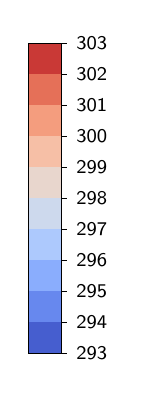
\begin{tikzpicture}[baseline=0pt,x=1cm,y=\figtenlegendunit]
            \fill[figtenTemp0] (0,0.00) rectangle (0.42,0.52);
            \fill[figtenTemp1] (0,0.52) rectangle (0.42,1.04);
            \fill[figtenTemp2] (0,1.04) rectangle (0.42,1.56);
            \fill[figtenTemp3] (0,1.56) rectangle (0.42,2.08);
            \fill[figtenTemp4] (0,2.08) rectangle (0.42,2.60);
            \fill[figtenTemp5] (0,2.60) rectangle (0.42,3.12);
            \fill[figtenTemp6] (0,3.12) rectangle (0.42,3.64);
            \fill[figtenTemp7] (0,3.64) rectangle (0.42,4.16);
            \fill[figtenTemp8] (0,4.16) rectangle (0.42,4.68);
            \fill[figtenTemp9] (0,4.68) rectangle (0.42,5.20);
            \draw[line width=0.35pt] (0,0) rectangle (0.42,5.20);
            \foreach \y/\ticklabel in {
                0.00/293,0.52/294,1.04/295,1.56/296,2.08/297,
                2.60/298,3.12/299,3.64/300,4.16/301,4.68/302,5.20/303}
                {\draw[line width=0.3pt] (0.42,\y) -- (0.49,\y)
                 node[anchor=west,font=\sffamily\fontsize{7.5}{8}\selectfont]
                 {\ticklabel};}
        \end{tikzpicture}%
    }

    \newcommand{\figtenpanellabel}[2]{%
        {\sffamily\bfseries\fontsize{8.5}{9.5}\selectfont
         (#1) $h_d/l_d=#2$}%
    }

    \begin{tabular}[c]{@{}l@{\hspace{0.10in}}c@{\hspace{0.05in}}c@{\hspace{0.05in}}c@{}}
        {\sffamily\bfseries\fontsize{8.5}{9.5}\selectfont Temperature} & & & \\[-1pt]
        \figtenlegendbar &
        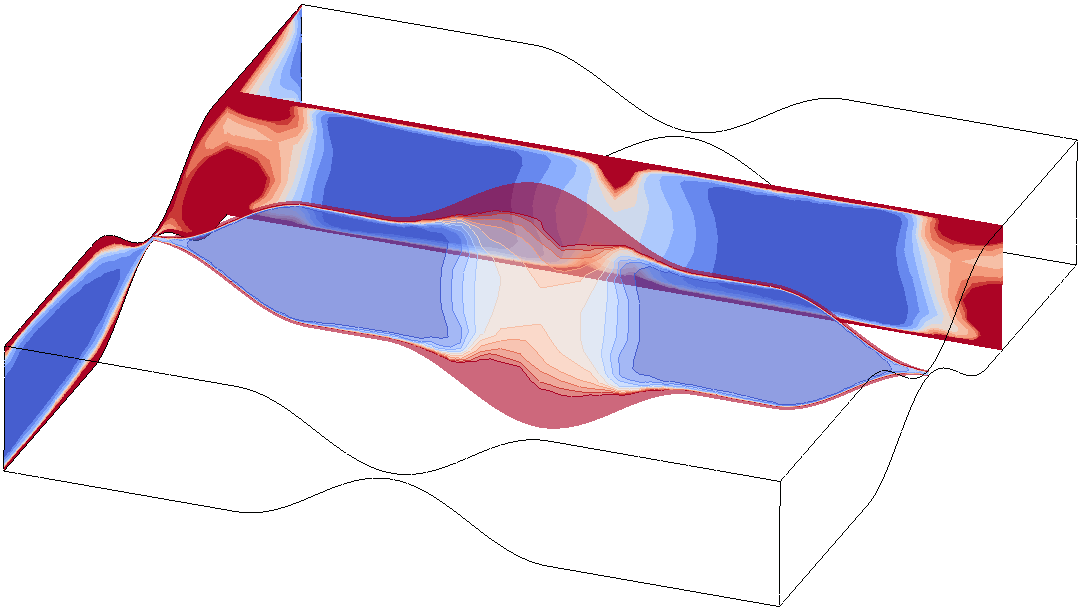
\includegraphics[width=\figtenpanelwidth]{image_2/Figure14/DH_2mm_Temp.png} &
        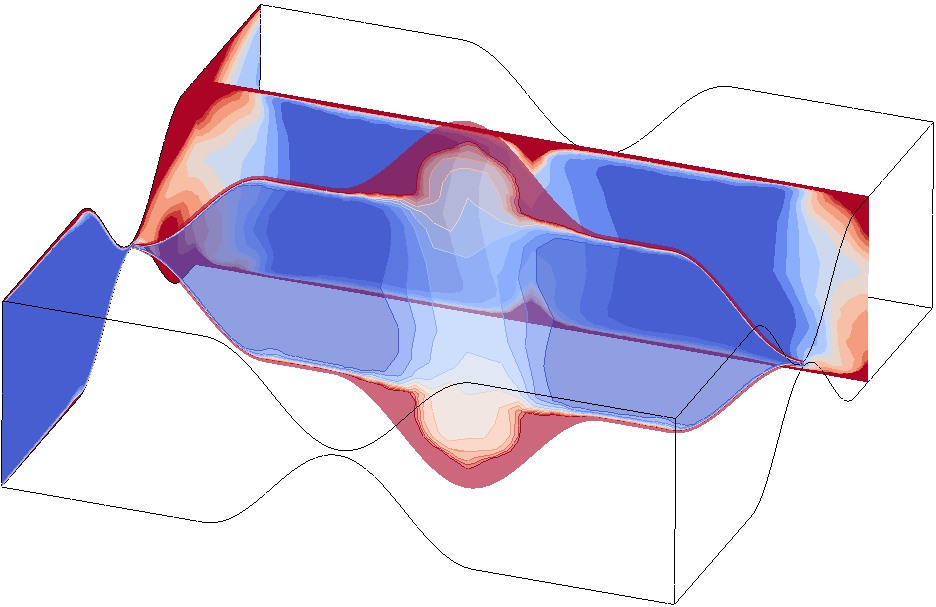
\includegraphics[width=\figtenpanelwidth]{image_2/Figure14/DH_3.5mm_Temp.png} &
        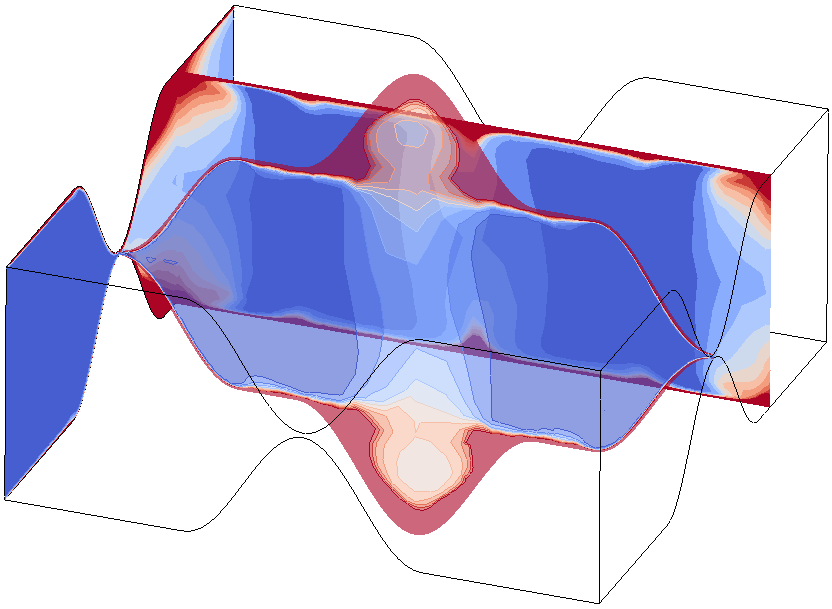
\includegraphics[width=\figtenpanelwidth]{image_2/Figure14/DH_5mm_Temp.png} \\[-1pt]
        {\sffamily\fontsize{7.5}{8.5}\selectfont $[\mathrm{K}]$} &
        \figtenpanellabel{a}{0.08} &
        \figtenpanellabel{b}{0.14} &
        \figtenpanellabel{c}{0.20}
    \end{tabular}
    \endgroup
    \caption{3D temperature distribution of DPHE at representative normalized dimple heights ($h_d/l_d=0.08$, $0.14$, and $0.20$).}
    \label{figure10}
\end{figure}
